\section{Test Results}
All integration checks within the integrated test {\tt SimScenarios/test\_scenarioIntegrators.py} passed.  Table~\ref{tbl:intResults} shows the test results, while Figure~\ref{fig:intResults} shows the resulting trajectories for each integration test.

\begin{figure}[t]
	\centerline{
	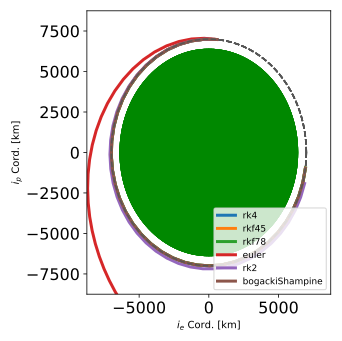
\includegraphics[]{../../../../SimScenarios/_Documentation/AutoTex/scenarioIntegrators}
	}
	\caption{Illustration of the BSK integrated trajectories.}
	\label{fig:intResults}
\end{figure}

\begin{table}[h]
	\caption{Integration test results.}
	\label{tbl:intResults}
	\centering \fontsize{10}{10}\selectfont
	\begin{tabular}{c | c | p{4in} } % Column formatting, 
		\hline\hline
		\textbf{Test} 			& \textbf{Pass/Fail} 	 & \textbf{BSK Error Notes} 									        
		\\ \hline
		``rk4"		  	& 
		\input{../../../../SimScenarios/_Documentation/AutoTex/scenarioIntegratorsTestMsg-rk4}      	  &
		\input{../../../../SimScenarios/_Documentation/AutoTex/scenarioIntegratorsMsg-rk4}
	         \\ \hline
		``euler''	   	           	&
		\input{../../../../SimScenarios/_Documentation/AutoTex/scenarioIntegratorsTestMsg-euler}           		&      
		\input{../../../../SimScenarios/_Documentation/AutoTex/scenarioIntegratorsMsg-euler}  
		\\ \hline
		``rk2''      	&
		\input{../../../../SimScenarios/_Documentation/AutoTex/scenarioIntegratorsTestMsg-rk2}
		   &  
		\input{../../../../SimScenarios/_Documentation/AutoTex/scenarioIntegratorsMsg-rk2}
\\ 
		\hline\hline
	\end{tabular}
\end{table}